\scanpage{117}
\mspage{20}
\uline{d'ouverts} $X'_i$, \uline{affines sur} $S'$, \uline{qui soient} ``\uline{stables}'' \uline{par la donnée de descente sur} $X'$. \margin{\figure{\begin{tikzpicture}\draw[gray] (-.09,.37)--(.08,.42);\draw[gray] (0,0)--(0,.4);\draw[gray] (-.08,-.04)--(.08,0);\end{tikzpicture}}} Il en est certainement ainsi (quelque soit $X'/S'$ et la donnée de descente sur $X'$) si le morphisme $\alpha:S'\longrightarrow S$ est \uline{radiciel} (i.e. injectif, \margin{\figure{\begin{tikzpicture}\draw[gray] (-.09,.37)--(.08,.42);\draw[gray] (0,0)--(0,.4);\draw[gray] (-.08,-.04)--(.08,0);\end{tikzpicture}}} et à extensions résiduelles \deleted{rad} qui sont radicielles). On peut montrer aussi qu'il en est encore ainsi si $\alpha:S'\longrightarrow S$ est \uline{fini}, et \deleted{\unsure{si}} toute partie finie de $X'$, contenue dans une fibre de $X'$ sur $S$, est contenue dans un ouvert \deleted{affine} de $X'$ affine sur $S\deleted{\unsure{_x}}$ (c'est le \uline{critère de} WEIL). \margin{\figure{\begin{tikzpicture}\draw[gray] (-.09,.37)--(.08,.42);\draw[gray] (0,0)--(0,.4);\draw[gray] (-.08,-.04)--(.08,0);\end{tikzpicture}}} Il en est en particulier ainsi si $X'/S'$ est quasi-projectif, et dans ce cas, on peut montrer que le préschéma ``descendu'' \deleted{$X$ sur $S$ est} $X/S$ est aussi quasi-projectif (et projectif si $X'/S'$ l'est).

En résumé:

\uuline{Théorème} 3 Soit $\alpha:S'\longrightarrow S$ un morphisme \inserted{de préschémas,} fidèlement plat et quasi-compact. Si $\alpha$ est \uline{radiciel}, c'est un \uline{morphisme de descente strict}. Si $\alpha$ est fini, c'est un morphisme de descente strict relativement à la catégorie fibrée des préschémas quasi-projectifs (ou projectifs) sur des préschémas.

\uuline{Remarques} J'ignore si dans la deuxième assertion ci-dessus, l'hypothèse que $\alpha$ soit un morphisme \uline{fini} est \deleted{vraiment essentielle} bien nécessaire; on vérifie en tous cas de façon \deleted{purement} ``formelle'' qu'on peut la remplacer par l'hypothèse suivante, plus faible en apparence: \inserted{pour} \uline{tout point de} $S$ \deleted{a} \inserted{existe} un \uline{voisinage ouvert} $U$, \uline{un} $U'$ \uline{fini et fidèlement plat} sur $U$, \uline{et un S-morphisme de} $U'$ \uline{dans} $S'$. Un cas type \deleted{\unsure{où}} qui ne rentre pas dans le précédent est celui où $S=\operatorname{Spec}(A)$, \margin{\figure{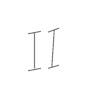
\begin{tikzpicture}\draw[gray] (-.08,.44)--(.08,.47) (0,0)--(0,.45) (-.08,-.03)--(.08,0);\draw[gray] (.22,.02)--(.25,.48) (.17,.46)--(.31,.51) (.17,0)--(.31,.04);\end{tikzpicture}}} $S'=\operatorname{Spec}(\bar A)$, où $A$ est un anneau local noethérien et $\bar A$ son complété; ou encore celui où $S'$ est quasi-fini sur $S$ (i.e. localement isomorphe à un ouvert d'un $S$-schéma fini) et non fini. Dans ces deux cas, \deleted{j'ignore en particulier} le conférencier ignore aussi la réponse à la question suivante: soit $X$ un $S$-schéma tel que $X'=X\times_S S'$ \margin{\figure{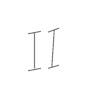
\begin{tikzpicture}\draw[gray] (-.08,.44)--(.08,.47) (0,0)--(0,.45) (-.08,-.03)--(.08,0);\draw[gray] (.22,.02)--(.25,.48) (.17,.46)--(.31,.51) (.17,0)--(.31,.04);\end{tikzpicture}}} soit projectif sur $S'$, est-il vrai que $X$ est projectif sur $S$ ?

2. \uline{Application à la descente de certaines propriétés de morphismes}.- \margin{\figure{\begin{tikzpicture}\draw[gray] (5.8,.2) .. controls (6.2,-.05) and (4.5,-.12) .. (1,-.12) .. controls (-.2,-.14) and (-.3,-.42) .. (0,-.45);\end{tikzpicture}}}

Soit $P$ une \deleted{propriété} \inserted{classe} de morphismes de préschémas. Soit $\alpha:S'\longrightarrow S$ un morphisme de préschémas, \deleted{soient $X,Y$ deux $S$} et soit $f:X\longrightarrow Y$ un morphisme de $S$-préschémas, $f':X'\longrightarrow Y'$ l'image réciproque de $f$ par $\alpha$. On peut se demander alors si la relation \deleted{``$f'$ satisfait $P$''} \inserted{``$f'\in P$''} implique \deleted{``$f$ satisfait} \inserted{``$f\in$} $P$''. \margin{\figure{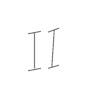
\begin{tikzpicture}\draw[gray] (-.08,.44)--(.08,.47) (0,0)--(0,.45) (-.08,-.03)--(.08,0);\draw[gray] (.22,.02)--(.25,.48) (.17,.46)--(.31,.51) (.17,0)--(.31,.04);\end{tikzpicture}}} Il apparaît que la réponse est affirmative dans beaucoup de cas importants lorsque l'on suppose que $\alpha$ est \uline{fidèlement plat} et \uline{quasi}
\margin{116}
